\documentclass[../mathNotesPreamble]{subfiles}
\begin{document}
%\relscale{1.4} %TODO
\section{17.3: Conservative Vector Fields}

  \begin{defn*}[Simple and Closed Curves]
    Suppose a curve $C$ (in $\bbr^2$ or $\bbr^3$) is described parametrically by $\vecr(t)$, where $a\leq t\leq b$. Then $C$ is a \textbf{simple curve} if $\vecr(t_1)\neq \vecr(t_2)$ for all $t_1$ and $t_2$, with $a<t_1<t_2<b$; that is, $C$ never intersects itself between its endpoints. The curve $C$ is \textbf{closed} if $\vecr(a)=\vecr(b)$; that is, the initial and terminal points of $C$ are the same.
  \end{defn*}
  \vspace*{\stretch{1}}

  \noindent
  \begin{minipage}{0.5\linewidth}
    \begin{center}
      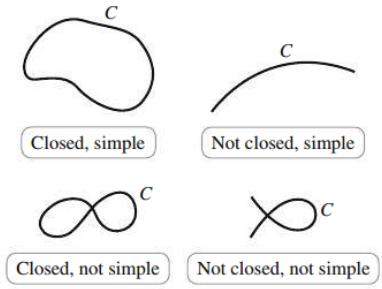
\includegraphics[width=0.9\linewidth]{../images/briggs_17_03/fig17_28}
    \end{center}
  \end{minipage}%
  \begin{minipage}{0.5\linewidth}
    \begin{center}
      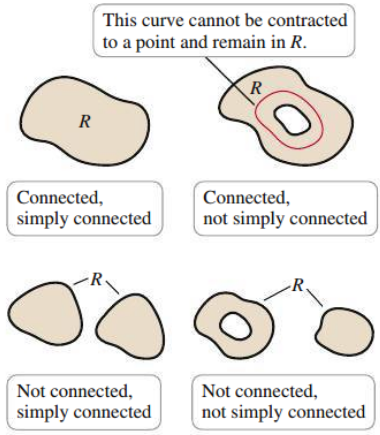
\includegraphics[width=0.8\linewidth]{../images/briggs_17_03/fig17_29}
    \end{center}
  \end{minipage}%
  \vspace*{\stretch{1}}

  \begin{defn*}[Connected and Simply Connected Regions]
    An open region $R$ in $\bbr^2$ (or $D$ in $\bbr^3$) is \textbf{connected} if it is possible to connect any two points of $R$ by a continuous curve lying in $R$. An open region $R$ is \textbf{simply connected} if every closed simple curve in $R$ can be deformed and contracted to a point in $R$.
  \end{defn*}
  \pagebreak

  \begin{defn*}[Conservative Vector Field]
    A vector field $\mathbf F$ is said to be \textbf{conservative} on a region (in $\bbr^2$ or $\bbr^3$) if there exists a scalar function $\varphi$ such that $\mathbf F=\grad\varphi$ on that region.
  \end{defn*}
  Assume that $\mathbf F=\bracket{f,g,h}$ is a conservative vector field. Then, there exists $\varphi$ such that
    \[\bracket{f,g,h}=\grad \varphi=\bracket{\varphi_x, \varphi_y, \varphi_z}\]
  Now, we consider the second partial derivatives:

  \noindent
  \begin{minipage}{0.25\linewidth}
    \begin{align*}
      \varphi_{xy}&= \varphi_{yx} \Rightarrow\\[\baselineskip]
      \varphi_{xz}&= \varphi_{zx} \Rightarrow\\[\baselineskip]
      \varphi_{yz}&= \varphi_{zy} \Rightarrow
    \end{align*}
  \end{minipage}
  \vspace*{\stretch{1}}

  \begin{thmBox*}[Theorem 17.3: Test for Conservative Vector Fields]
    Let $\mathbf F=\bracket{f,g,h}$ be a vector field defined on a connected and simply connected region $D$ of $\bbr^3$, where $f$, $g$, and $h$ have continuous first partial derivatives on $D$. Then $\mathbf F$ is a conservative vector field on $D$ (there is a potential function $\varphi$ such that $\mathbf F=\grad \varphi$) if and only if
      \[\frac{\partial f}{\partial y}=\frac{\partial g}{\partial x},\qquad
      \frac{\partial f}{\partial z}=\frac{\partial h}{\partial x},\qquad
      \textnormal{and } \quad\frac{\partial g}{\partial z}=\frac{\partial h}{\partial y}.\]
    For vector fields in $\bbr^2$, we have the single condition $\ds\frac{\partial f}{\partial y}=\frac{\partial g}{\partial x}$.
  \end{thmBox*}
  \pagebreak

  \begin{ex*}
    Determine if the following vector fields are conservative:
  \end{ex*}
  \begin{tasks}[after-item-skip=\stretch{1}, label=](1)
    \task $\mathbf F=\bracket{e^x\cos(y),-e^x\sin(y)}$
    \task $\mathbf F=\bracket{2xy-z^2, x^2+2z, 2y-2xz}$
  \end{tasks}
  \vspace*{\stretch{1}}
  \pagebreak

  \begin{thmBox*}[Procedure: Finding Potential Functions in $\bbr^3$]
    Suppose $\mathbf F=\bracket{f,g,h}$ is a conservative vector field. To find $\varphi$ such that $\mathbf F=\grad \varphi$, use the following steps:
    \begin{enumerate}
      \item 
        Integrate $\varphi_x=f$ with respect to $x$ to obtain $\varphi$, which includes an arbitrary function $c(y,z)$.
      \item 
        Compute $\varphi_y$ and equate it to $g$ to obtain an expression for $c_y(y,z)$.
      \item 
        Integrate $c_y(y,z)$ with respect to $y$ to obtain $c(y,z)$, including an arbitrary function $d(z)$.
      \item 
        Compute $\varphi_z$ and equate it to $h$ to get $d(z)$.
    \end{enumerate}
    A similar procedure beginning with $\varphi_y=g$ or $\varphi_z=h$ may be easier in some cases.
  \end{thmBox*}

  \begin{ex*}
    Find a potential function for the following conservative vector fields:
  \end{ex*}
  \begin{tasks}[after-item-skip=\stretch{1}, label=](1)
    \task $\mathbf F=\bracket{e^x\cos(y),-e^x\sin(y)}$
  \end{tasks}
  \vspace*{\stretch{1}}
  \pagebreak

  \begin{tasks}[after-item-skip=\stretch{1}, label=](1)
    \task $\mathbf F=\bracket{2xy-z^2, x^2+2z, 2y-2xz}$
  \end{tasks}
  \vspace*{\stretch{1}}
  \pagebreak

  \noindent\textbf{Fundamental Theorem for Line Integrals and Path Independence:}

  \noindent Suppose that $\mathbf F$ is a conservative vector field in $\bbr^3$ with potential function $\varphi$. 
  \begin{align*}
    \frac{d\varphi}{dt}&= \frac{\partial\varphi}{\partial x}\frac{dx}{dt}+\frac{\partial\varphi}{\partial y}\frac{dy}{dt}+\frac{\partial\varphi}{\partial z}\frac{dz}{dt}\\
      &=\bracket{\frac{\partial \varphi}{\partial x},\frac{\partial \varphi}{\partial y},\frac{\partial \varphi}{\partial z}}\cdot\bracket{\frac{dx}{dt},\frac{dy}{dt},\frac{dz}{dt}}\\
      &=\grad\varphi\cdot\vecr'(t)\\
      &=\mathbf F\cdot\vecr'(t),
  \end{align*}
  where $\vecr(t)$ defines a curve $C$ for $a\leq t\leq b$. Now, we integrate $\mathbf F$ over the curve $C$:
  \begin{align*}
    \int_C\mathbf F\cdot d\vecr= \int_a^b \mathbf F\cdot\vecr'(t)\,dt
      =\int_a^b \frac{d\varphi}{dt}\,dt
      =\varphi(B)-\varphi(A)
  \end{align*}
  where $A$ and $B$ are points corresponding to $\vecr(a)$ and $\vecr(b)$ respectively.
  \vspace*{\stretch{1}}


  \begin{thmBox*}[Theorem 17.4: Fundamental Theorem for Line Integrals]
    Let $R$ be a region in $\bbr^2$ or $\bbr^3$ and let $\varphi$ be a differentiable potential function defined on $R$. If $\mathbf F=\grad\varphi$ (which means that $\mathbf F$ is conservative), then
       \[\int_C \mathbf F\cdot\vecT\,ds=\int_C \mathbf F\cdot d\vecr=\varphi(B)-\varphi(A),\]
     for all points $A$ and $B$ in $R$ and all piecewise-smooth oriented curves $C$ in $R$ from $A$ to $B$.
  \end{thmBox*}

  \begin{defn*}[Independence of Path]
    Let $\mathbf F$ be a continuous vector field with domain $R$. If $\int_{C_1} \mathbf F\cdot d\vecr=\int_{C_2} \mathbf F\cdot d\vecr$ for all piecewise-smooth curves $C_1$ and $C_2$ in $R$ with the same initial and terminal points, then the line integral is \textbf{independent of path}.
  \end{defn*}
  \pagebreak

  \begin{thmBox*}[Theorem 17.5]
    Let $\mathbf F$ be a continuous vector field on an open connected region $R$ in $\bbr^2$. If $\int_C \mathbf F\cdot d\vecr$ is independent of path, then $\mathbf F$ is conservative; that is, there exists a potential function $\varphi$ such that $\mathbf F=\grad \varphi$ on $R$. 
  \end{thmBox*}

  \begin{ex*}
    Consider the potential function $\varphi(x,y)=\parens{x^2-y^2}/2$ with gradient field $\mathbf F=\bracket{x,-y}$.
    \begin{itemize}
      \item Let $C_1$ be the quarter-circle $\vecr(t)=\bracket{\cos(t),\sin(t)}$, for $0\leq t\leq \pi/2$, from $A(1,0)$ to $B(0,1)$,
      \item let $C_2$ be the line $\vecr(t)=\bracket{1-t,t}$, for $0\leq t\leq 1$, also from $A$ to $B$.
    \end{itemize}
    Evaluate the line integrals of $\mathbf F$ on $C_1$ and $C_2$, and show that both are equal to $\varphi(B)-\varphi(A)$.
  \end{ex*}
  \vspace*{\stretch{1}}
  \pagebreak

  \begin{ex*}
     With $\mathbf F=\bracket{y-x,\,x}$ on the following oriented paths in $\bbr^2$.
  \end{ex*}
  \vspace*{-\baselineskip}
  \noindent
  \begin{minipage}[t]{0.6\linewidth}\mbox{}
    \begin{tasks}[after-item-skip=8\baselineskip, label=\alph*)](1)
      \task 
        Find the potential function $\varphi(x,y)$
    \end{tasks}
  \end{minipage}
  \begin{minipage}[t]{0.4\linewidth}\mbox{}
    \begin{flushright}
      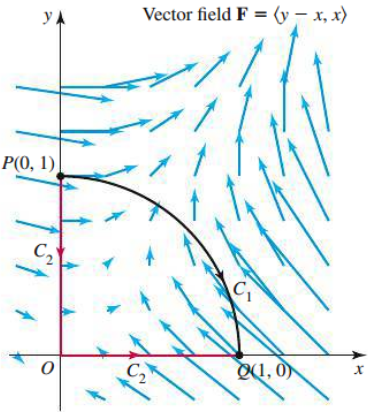
\includegraphics[width=0.75\linewidth]{../images/briggs_17_02/fig17_20}
    \end{flushright}
  \end{minipage}
  \begin{tasks}[after-item-skip=\stretch{1}, label=\alph*), resume](1)
    \task 
      Evaluate $\int_C \mathbf F\cdot d\vecr$ along
      \begin{enumerate}[itemsep=6\baselineskip, label=]
        \item 
          the quarter-circle $C_1$ from $P(0,1)$ to $Q(1,0)$,
        \item 
          the path $C_2$ from $P(0,1)$ to $Q(1,0)$ via two line segments through $O(0,0)$.
      \end{enumerate}
  \end{tasks}
  \vspace*{\stretch{1}}
  \pagebreak

  \begin{ex*}
    Evaluate
      \[\int_C \bracket{2xy-z^2,\, x^2+2z,\,2y-2xz}\,d\vecr\]
    where $C$ is the curve from $A(-3,-2,1)$ to $B(1,2,3)$.
  \end{ex*}
  \vspace{\stretch{1}}
  \pagebreak

  \begin{thmBox*}[Theorem 17.6: Line Integrals on Closed Curves]
    Let $R$ be on open connected region in $\bbr^2$ or $\bbr^3$. Then $\mathbf F$ is a conservative vector field on $R$ if and only if $\oint_C \mathbf F\cdot d\vecr=0$ on all simple closed piecewise-smooth oriented curves $C$ in $R$.
  \end{thmBox*}

  \begin{ex*}
    Evaluate $\displaystyle \int_C \bracket{2xy+z^2,\,x^2,\,2xz}\cdot d\vecr$ where $C$ is the circle \newline$\vecr(t)=\bracket{3\cos(t),\,4\cos(t),\,5\sin(t)}$, for $0\leq t\leq 2\pi$.
  \end{ex*}

  \pagebreak
  
\end{document}
